% INTRO PCA CONCEPTS

\section[Introduction]{Introduction} % Sectio
%\begin{frame}
%    \frametitle{Principal Component Analysis} % Slide title%
%	\textbf{Purpose}
%	\begin{itemize}
%		\item Principal component space of lower dimension than the initial space
%	\end{itemize}
%
%	\textbf{Steps}
%	\begin{itemize}
%		\item Build the covariance matrix $\bar{C}$
%		\item Calculate the \textit{N} eigenvectors corresponding to the highest eigenvalues obtained by diagonalization of $\bar{C}$
%		\item The representation of X in the principal component space is $Y = PX$, with the rows of P composed of the \textit{eigenvectors} maximizing the variance
%	\end{itemize}
%\end{frame}

\begin{frame}
    \frametitle{Kernel Principal Component Analysis: Motivation} % Slide title
	Take non-linearities into account\\
	\vspace{0.5cm}
	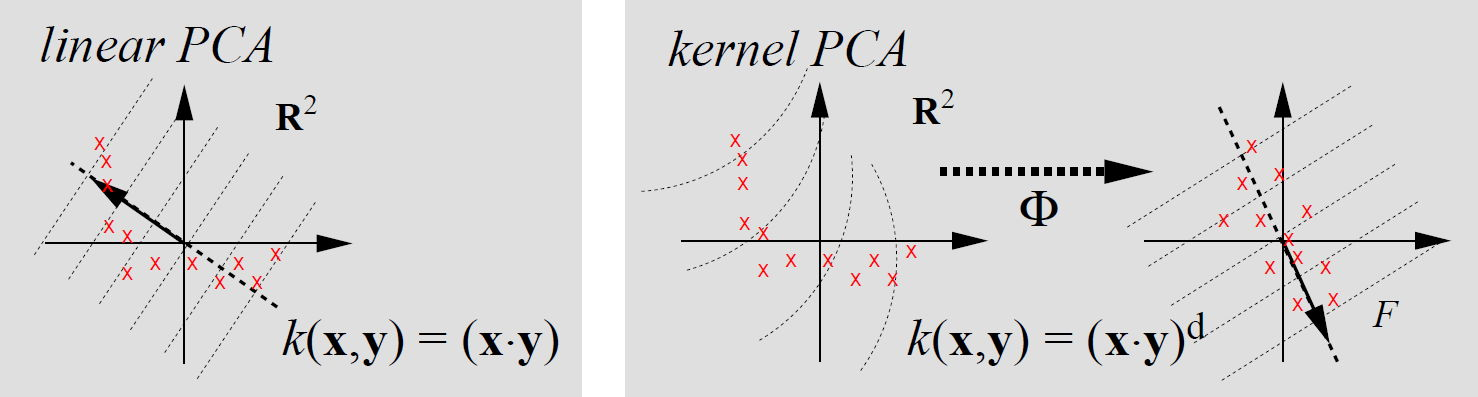
\includegraphics[width=0.8\textwidth]{build/kernel_pca.jpg}    
	
		\begin{itemize}
		\item \textit{PC} are extracted from the high-dimension feature space F
		\item Kernel functions gives us $\Phi(\textbf{x}) \cdot \Phi(\textbf{y})$ for a low computation cost
	\end{itemize}
   
\end{frame}

%    
%	\begin{itemize}
%		\item \textit{PC} are extracted from the high-dimension feature space F which 
%		\item  $\Phi : \mathbb{R}^N \rightarrow F, \textbf{x} \rightarrow \textbf{X}$
%		\item Kernel functions gives us $\Phi(\textbf{x}) \cdot \Phi(\textbf{y})$ for a low computation cost
%	\end{itemize}
